\section{Introduction}

\begin{figure*}[t]
\centering
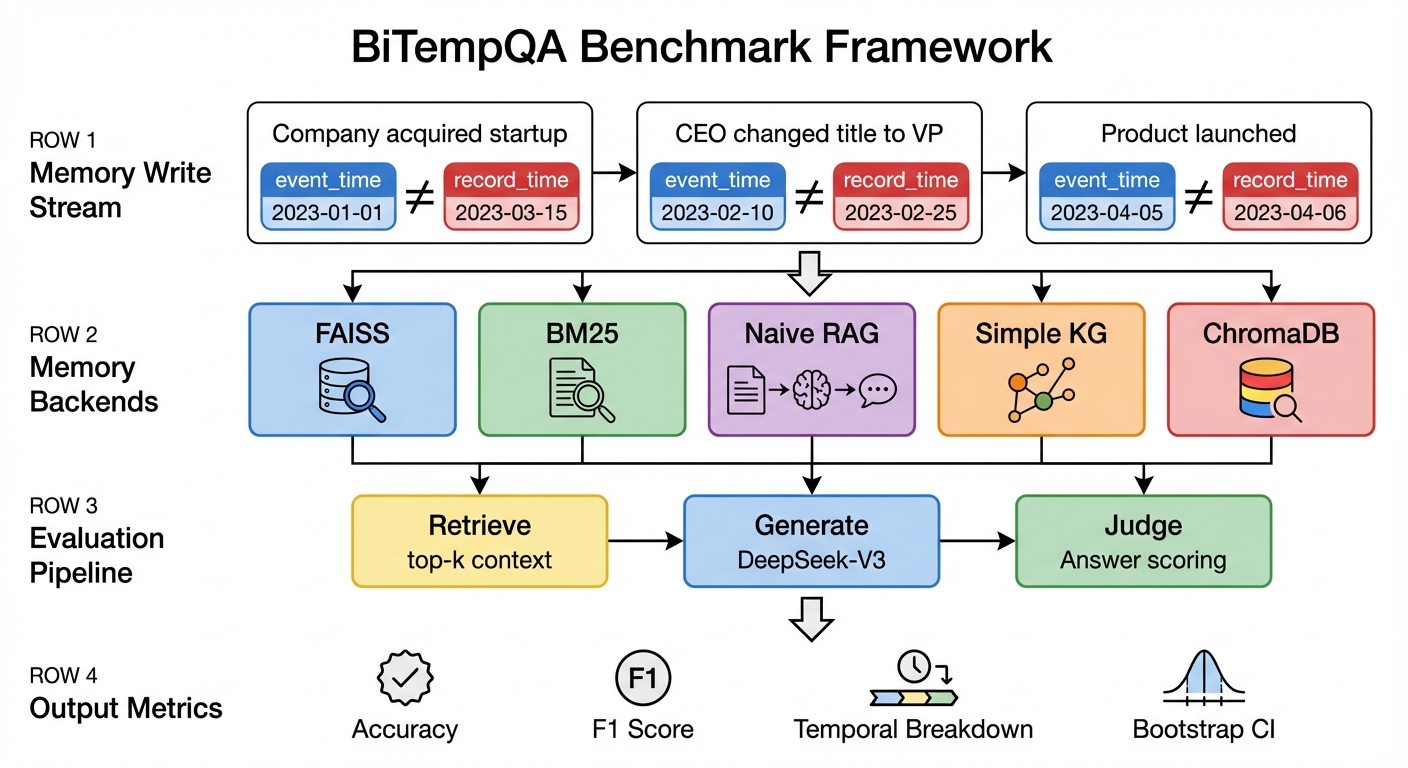
\includegraphics[width=\textwidth]{figures/fig1_framework.jpeg}
% 中文注释：caption 保留原意，但把语气调整得更自然、更符合论文写法。
\caption{BiTempQA framework overview. Each memory write carries dual timestamps: \textcolor{blue}{event time}, indicating when the event occurred, and \textcolor{red}{record time}, indicating when the system recorded it. Five memory backends retrieve context, which is then processed in a unified Retrieve $\rightarrow$ Generate $\rightarrow$ Judge pipeline to produce diagnostic metrics.}
\label{fig:framework}
\end{figure*}

Consider a medical AI assistant that learns at 10:00~AM on Tuesday that a patient's symptoms began two days earlier.
% 中文注释：这里保留必要斜体强调，但把举例句式改得更严谨，减少口语感。
To answer ``What was the patient's status on Sunday morning?'' correctly, the system must distinguish \emph{when the symptoms started} (event time) from \emph{when the system recorded this fact} (record time).
This bitemporal distinction, well established in temporal database theory~\citep{snodgrass1999tsql2,jensen1999temporal}, arises in many settings: financial trades execute on Monday but settle on Wednesday, news events occur on Thursday evening but are reported on Friday morning, and scientific findings may be established in 2022 but published in 2024.
A memory system that conflates these timestamps is therefore likely to make incorrect temporal inferences.

Despite its practical importance, this capability is not systematically evaluated in existing benchmarks for LLM-based memory systems.
Temporal reasoning benchmarks such as \textsc{TimE}~\citep{time2025}, \textsc{ETRQA}~\citep{etrqa2024}, and \textsc{Test of Time}~\citep{testoftime2025} primarily study reasoning over static text rather than over dynamically evolving memory stores.
Memory-system benchmarks such as LoCoMo~\citep{locomo2024}, LongMemEval~\citep{longmemeval2024}, and MemoryAgentBench~\citep{memoryagentbench2025} include temporal questions, but they generally treat time as a single dimension and do not distinguish event occurrence from information acquisition.
% 中文注释：把“我们无法诊断”改成更客观的“仍难以判断”，语气更符合学术论文。
As a result, it remains difficult to determine whether failures on temporal questions arise primarily from \emph{retrieval limitations} or \emph{reasoning limitations}, and which temporal reasoning types are most challenging.

We present BiTempQA, a diagnostic benchmark designed to address this gap.
BiTempQA is grounded in a central idea from bitemporal data modeling: each fact has two independent temporal dimensions.
% 中文注释：这里收紧数据介绍的语气，同时保留所有原始统计信息不变。
The benchmark contains 1,536 Chinese QA pairs, including a 308-item held-out test set, spanning 10 scenario types across 6 domains, with 9 question types at 3 difficulty levels.
Each memory write carries explicit event-time and record-time annotations, and 56.5\% of questions require reasoning about both timestamps simultaneously.
We evaluate five memory backends (FAISS, BM25, Naive RAG, Simple Knowledge Graph, and ChromaDB) in a unified Retrieve $\rightarrow$ Generate $\rightarrow$ Judge pipeline.

Our contributions are as follows.
First, we introduce, to our knowledge, the first dual-timestamp diagnostic benchmark for memory systems, with explicit event-time and record-time annotations on every memory write and structured metadata on every question.
% 中文注释：这里把 claim 改成更可辩护的学术语气，避免把统计关联直接写成过强结论。
Second, we show that record-time reasoning is associated with lower accuracy than event-time reasoning ($p = 0.023$ in a mixed-effects regression controlling for question type, difficulty, and scenario), supporting the benchmark's diagnostic usefulness.
Third, we report several diagnostic findings: sampled failures appear primarily retrieval-related ($\sim 55\%$), confidence is often poorly calibrated (AUROC $< 0.5$ for some systems), and memory backends exhibit substantial complementarity (oracle +9.8pp over the best single system).
Fourth, we compare BiTempQA with LoCoMo~\citep{locomo2024} and find that graph-based memory is relatively strong on adversarial robustness (97.5\%) but comparatively weak on temporal reasoning (37.5\%).
